%!TEX root = <main.tex>
\section{Optimizations}

In this section we explain \textit{incremental inference} and \textit{approximate inference} in detail.
In \system~ these optimizations are applied on top of the current dominant approach of performing occlusion experiment by performing CNN inference on batches of images where each image corresponds to an occluded instance of the original image.
Performing CNN inference on batches of images is important as it reduces per image inference time by amortizing the fixed overheads.
This simple optimization alone can give up to ~1.4X speedups on CPU environments and ~2X speedups on the GPU environment.
Finally we explain how \system~ configures it's internal system configurations for \textit{approximate inference} by using a sample image set during the initial tuning stage. 

\subsection{Incremental Inference}\label{sec:inc_computation}

As explained earlier, occlusion experiments in it's naive form performs many redundant computations.
In order to avoid these redundancies layers in a CNN has to be change aware i.e. reuse previous computations as much as possible and compute only the required ones.
In this section we focus on transformations that operate on a local spatial context (e.g. Convolution and Pooling) and explain how they can be modified to operate in a change aware manner.
The choice of CPUs vs GPUs for CNN inference also brings up new considerations for the implementation of change aware CNN transformations and we explain two version of implementations, one which is a naive implementation of incremental inference approach and the other a GPU optimized implementation.
We also explain change aware implementations of two other linear algebra operators, activation volume addition and concatenation, which are also two popular operators seen in CNN architectures.

\vspace{2mm}
\noindent \textbf{Change aware implementation of transformations that operate on a local spatial context.} 
The coordinates of the modified patch in the output activation volume of a transformation that operate on a local spatial context caused by a modified patch in the input activation volume are determined by the coordinates and the dimensions of the input patch, sizes of the filter kernel ($H_k$ and $W_k$), padding values ($P_x$ and $P_y$), and the strides ($S_x$ and $S_y$).
For example consider simplified demonstration shown in figure 


\begin{figure}[t]
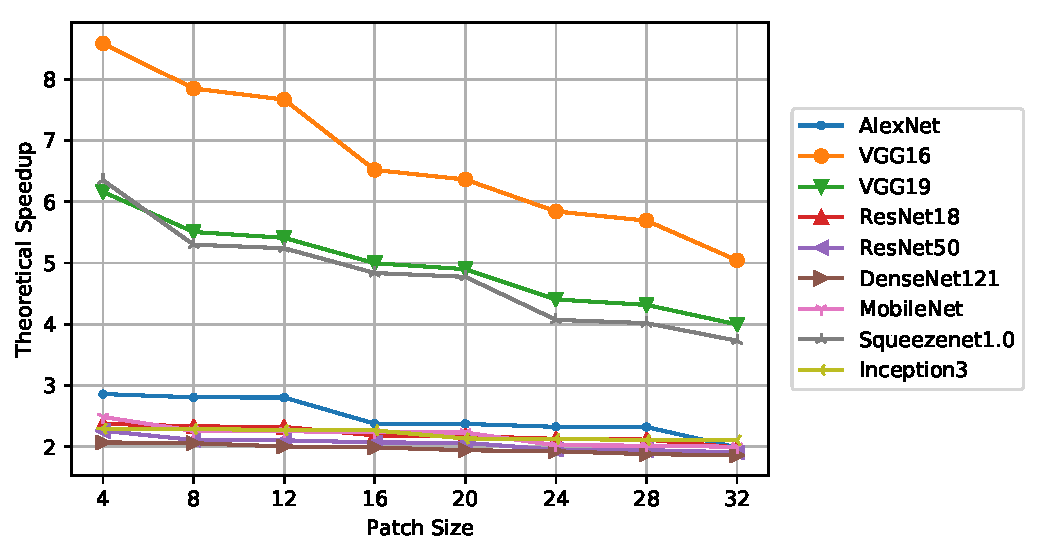
\includegraphics[width=\columnwidth]{images/redundancy_ratio}
\caption{Maximum attainable redundancy ratios of popular CNN architectures when a square occlusion patch of different sizes is placed on the center of the image.}
\label{fig:redundancy_ratio}
\end{figure}

Figure \ref{fig:redundancy_ratio} shows how the maximum attainable redundancy ratio changes for popular CNN architectures when a square occlusion patch of different sizes is placed on the center\footnote{If the occlusion patch is placed towards to a corner of the input image the redundancy ratio will be slightly higher. But placing the occlusion on the center gives us a worst case estimate.} of the input image. VGG 16 layer version results in the maximum redundancy ratio and Inception V3 model has the lowest redundancy ratio. Most CNN architectures results in a redundancy ratio between 2-3 except VGG 16, VGG 19, and Squeezenet 1.0 CNNs which results in higher redundancy ratios. The attainable redundancy ratio of a CNN is determined by the aspects of it's internal architecture such as number of layers, the size of the filter kernels, and the filter stride values.

\subsection{Approximate Inference}

\subsubsection{Adaptive Drill-Down}

\subsubsection{Patch Propagation Thresholding}

\subsection{System Tuning}
